\newpage

\section{Einführung}

	\subsection{Beschreibung}
		Die Idee hinter dem Projekt "SaveYourClicks" ist, wie der Name schon andeutet, dem alltäglichem User des Internets zu helfen Klicks und Zeit einzusparen. Dies soll daraus resultieren das eine Single Page Application (SPA) gegeben ist, die aus mehreren Widgets besteht. Jedes dieser Widgets soll eine kleine Funktion bieten (wie z.B. Wetteranzeige oder die momentanen Schlagzeilen aus Deutschland) und jeder User kann für sich selbst entscheiden welche Elemente er angezeigt haben möchte. So müssen nicht viele verschiedene Webseiten aufgerufen werden um minimale Informationen zu erhalten. 
		Außerdem soll die Möglichkeit bestehen eigenständige Widgets zu entwickeln und auf der Website zu veröffentlichen um so eine größere Vielfalt von Funktionen zu bieten.
	
	\subsection{Ziele}
	
		\subsubsection{Allgemein}
			Die Motivation der Website besteht darin dem einfachen Internetuser das Leben einfacher zu machen. Deswegen ist die Seite auch nicht für Firmen oder andere größere Einrichtungen gedacht. Durch die öffentliche Erweiterbarkeit ist der Umfang theoretisch Unbegrenzt, da jeder etwas beisteuern kann.
			
		\subsubsection{Marktanforderungen}  
			Die Website muss einfach zu bedienen sein und so simpel wie möglich gehalten werden. Da mehrere Widgets auf eine Seite vorhanden sein können, muss auch drauf geachtet werden das der Bildschirm nicht mit unnötigen Informationen überflutet wird. Die individuelle Einrichtung der Website muss auch noch nach einem erneuten Aufruf bestehen bleiben und darf nicht wieder zurückgesetzt werden.
			
		\subsubsection{Alleinstellungsmerkmale}  
			Nach bisheriger Recherche gibt es bis jetzt keine Webseiten die eine ähnliche Funktion bieten und somit sind alle Funktionen Alleinstellungsmerkmale.   
			
		\subsubsection{Zielgruppen}
			Hauptsächlich werden zwei Zielgruppen betrachtet: \\
			\textbf{Einfacher User: } Diese Zielgruppe benutzt nur die rudimentären Funktionen der Website. Sie hat eine große Variation von Menschen mit vielen verschieden Merkmalen.\\
			\textbf{Entwickler: }Diese Zielgruppe möchte neben herkömmlicher Nutzung der Website auch Widgets selbst Entwickeln und veröffentlichen. Sie hat allgemeine Kenntnisse zur JavaScript Entwickelung und hat schon eigene Webprojekte erstellt. Diese Gruppe kann von Hobbyentwickler bis hin zu professionellen Webentwicklern bestehen.   
			
		\subsubsection{Abgrenzung} 
			Die Website dient nicht dazu viele Webseiten in eins zu verschmelzen und darzustellen, sondern lediglich einen sehr geringen Teil an Informationen anzuzeigen. Außerdem sollen die Funktionen der einzelnen Widget so gering wie möglich gehalten werden und keine komplexen Daten enthalten um eine möglichst saubere GUI zu bieten. Das Softwaresystem dient auch nicht als Lesezeichenverwaltung oder soll eine Vorschau zu jeweiligen Webseiten fungieren.

\newpage				
\section{Anforderungen}

	\subsection{Funktionale Anforderungen}
		An das Programm werden die folgenden Anforderungen gestellt: 
		\begin{itemize}
			\item Bevor die Seite benutzt wird muss sich der User anmelden 
			\item Um sich anzumelden muss vorher eine Registrierung mit E-Mail und Passwort stattfinden  
			\item Auf der Startseite werden die Widgets angezeigt
			\item Über das angemeldete Konto kann man seine persönlichen Widgets einstellen und verwalten
			\item Falls gewollt kann das momentane Passwort geändert werden
			\item Es besteht die Möglichkeit seinen Account zu löschen und alle Daten von der Seite zu entfernen 
			\item Widgets können über die Einstellungen hinzugefügt oder entfernt werden
			\item Es können neue Widgets aus der Datenbank hinzugefügt werden um diese auf der Website zu benutzen 
			\item Nach der Abmeldung und dem Verlassen der Seite sollen alle Einstellungen gespeichert werden, damit beim erneuten Aufruf alle persönlichen Merkmale erhalten bleiben   
			\item User können ihre eigenen Widgets programmieren und auf der Website veröffentlichen    
		\end{itemize}
	
	\subsection{Nicht-funktionale Anforderungen}
		Neben den Funktionalen Anforderungen bestehen noch folgende Nicht-funktionale:
		\begin{itemize}
			\item Widgets sollen sehr knapp gehalten werden
			\item Einfache Navigierung der Website
			\item Schnelle Reaktionszeit der Elemente der Website
			\item Website entspricht den Usability Standards
			\item Die Seite soll für den Desktop optimiert sein
			\item Es soll nur eine bestimmte Anzahl an Widgets auf der Seite angezeigt werden
		\end{itemize}
	
		\subsubsection{Rahmenbedingungen}
		
		\subsubsection{Betriebsbedingungen}
		
		\subsubsection{Qualitätsmerkmale}
		
	\subsection{Graphische Benutzerschnittstelle}
		
		\subsubsection{Anmeldung}
			\begin{figure}[H]
				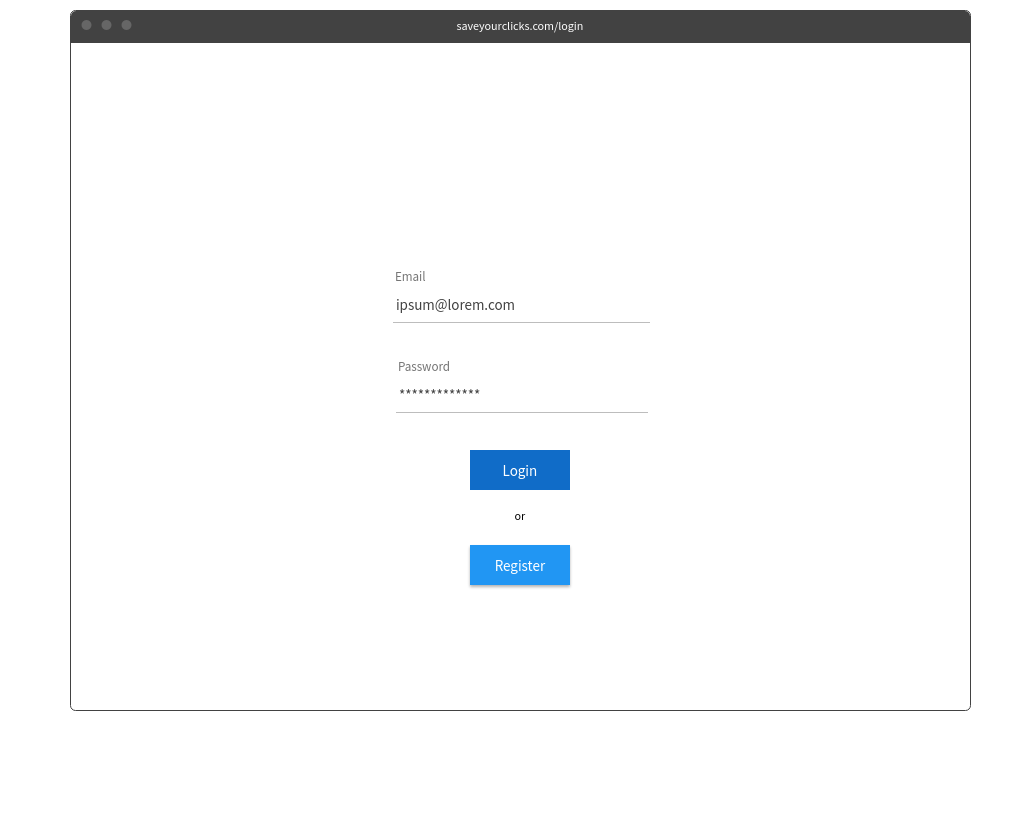
\includegraphics[scale=0.4]{images/p1}
			\end{figure}
		
		\subsubsection{Registrierung}
			\begin{figure}[H]
				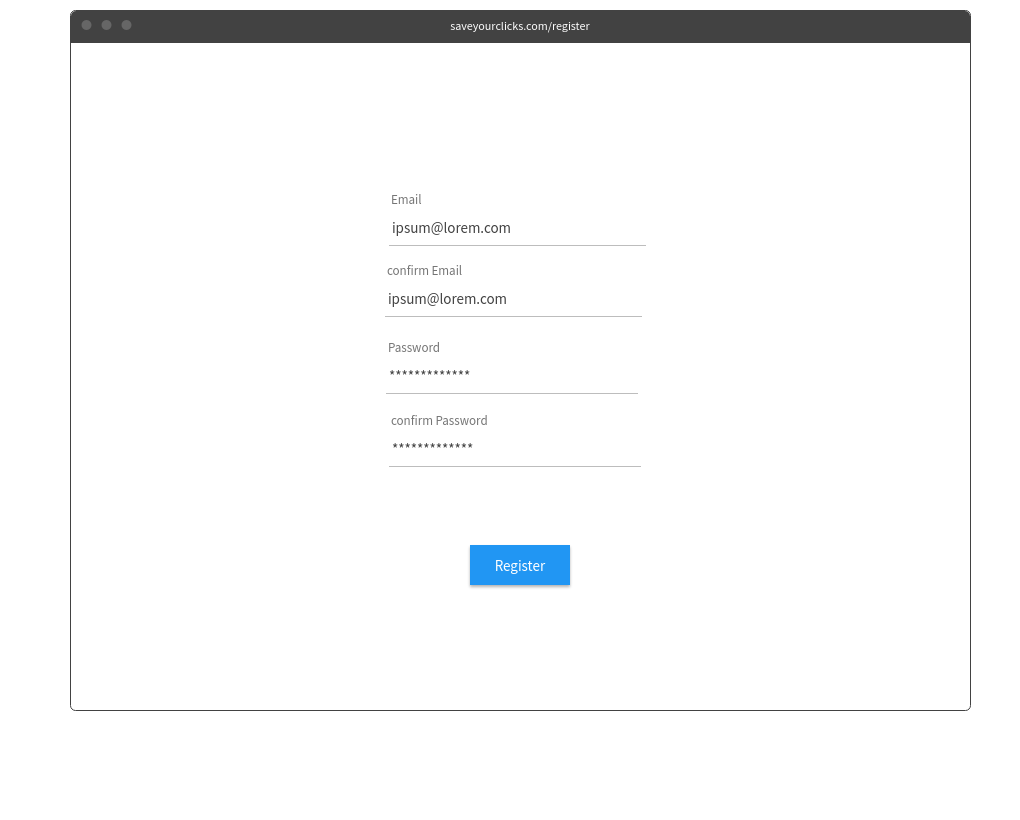
\includegraphics[scale=0.4]{images/p1reg}
			\end{figure}
		
		\subsubsection{Startseite}
			\begin{figure}[H]
				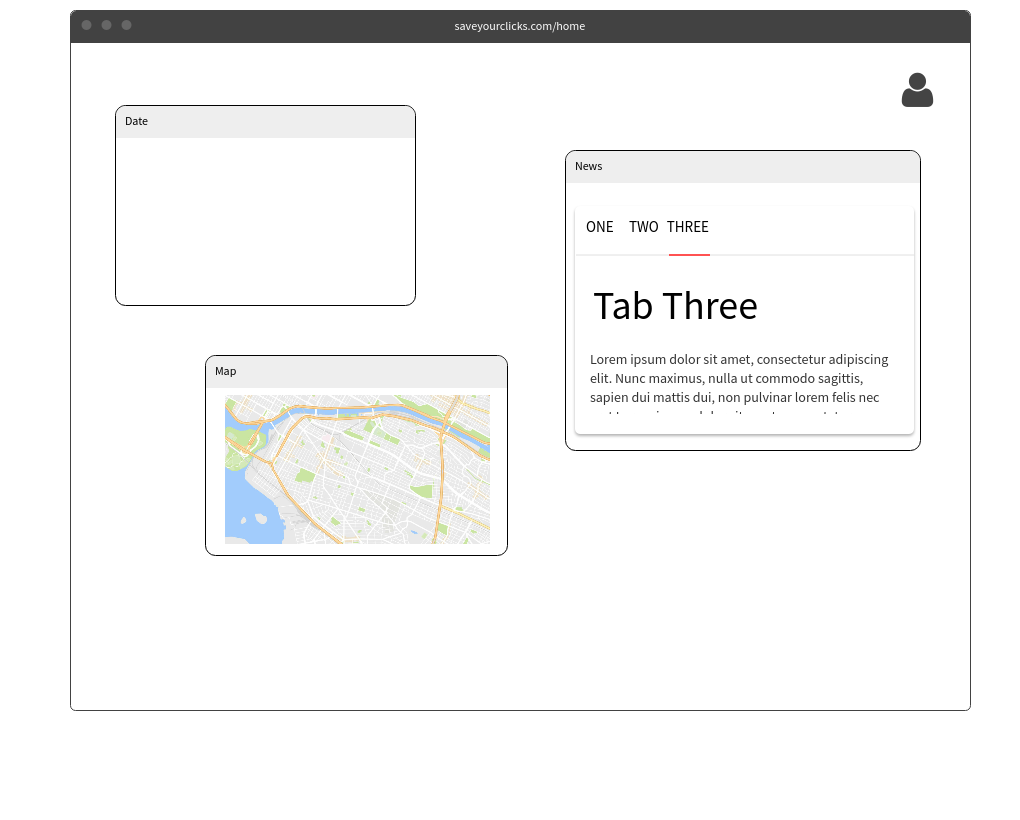
\includegraphics[scale=0.4]{images/p2}
			\end{figure}
		
		\subsubsection{Einstellungen}
			\begin{figure}[H]
				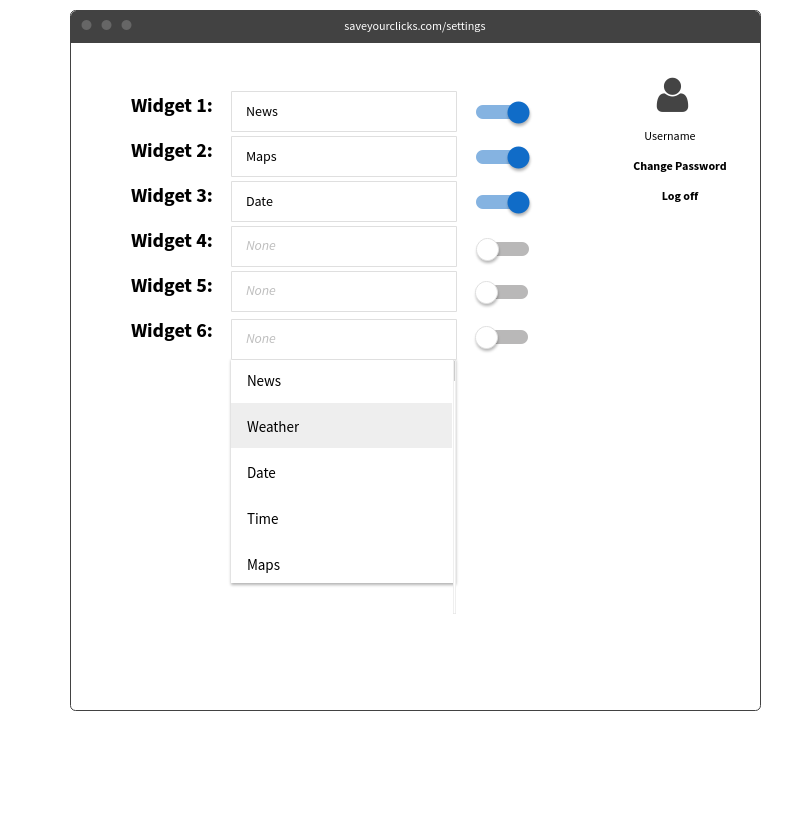
\includegraphics[scale=0.5]{images/p3}
			\end{figure}
		
		\subsubsection{Fileupload}
			\begin{figure}[H]
				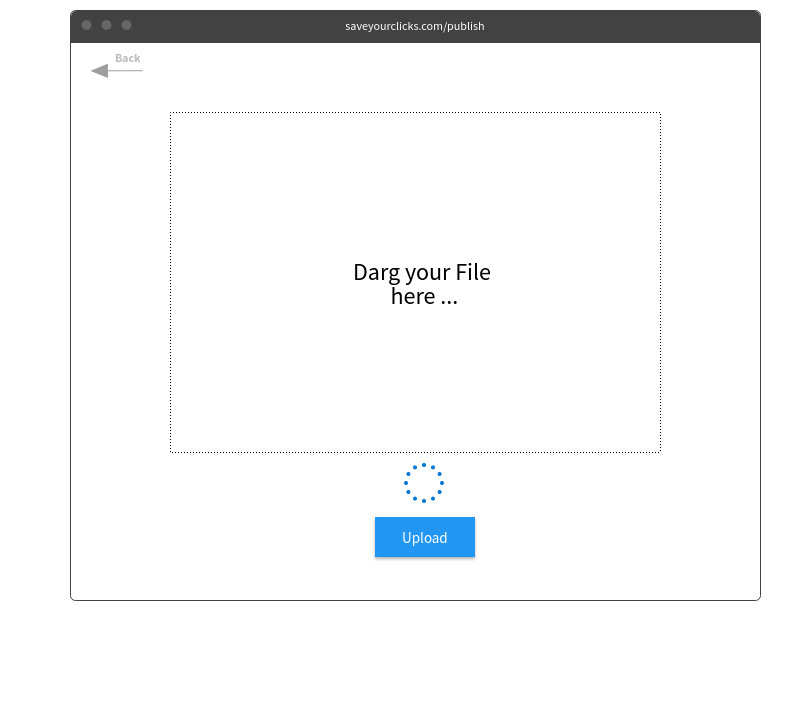
\includegraphics[scale=0.5]{images/p4}
			\end{figure}
		
		\subsubsection{Zustandsdiagramm}
			\begin{figure}[H]
				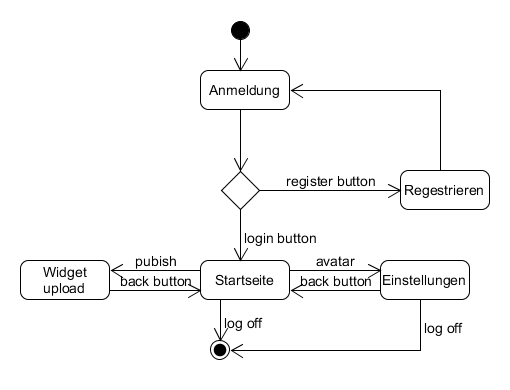
\includegraphics[scale=0.8]{images/zustand}
			\end{figure}
	
	\subsection{Anforderungen im Detail}
		
		\begin{center}
			\begin{tabular}{ | p{2cm} | p{2cm} | p{3cm} | p{3cm} | p{4cm} |}
				\hline
				\textbf{Name} & \textbf{Rolle} & \textbf{möchte ich} & \textbf{so dass} & \textbf{Akzeptanzkriterien}\\ \hline
				Registrieren & Besucher & mich registrieren & ich einen Account habe & Besucher gibt valide Daten an \\  \hline
				Anmelden & Besucher & mich Anmelde & ich meine persöhnliche \newline Seite bearbeiten kann & Der Besucher hat einen Account \\  \hline
				Abmelden & User & mich Abmelden & nicht mehr eingeloggt bin & Der Besucher ist angemeldet \\ \hline
				Widget hinzufügen & User & ein Widget hinzugügen & das Widget auf meinem Desktop angezeigt wird & Das Widget wird Angeboten und der User ist angemeldet \\ \hline
				Widget entfernen & User & ein Widget entfernen & das Widget nicht mehr angezeigt wird & Das Widget war hinzugefügt und der User ist angemeldet \\ \hline
				Neues Widget erstellen & Entwickler & ein Widget erstellen & ich und andere dieses Widget nutzen können & Das Widget entspricht den Vorgaben \\ \hline
				Widget zulassen & Admin & ein neues Widget zulassen & die User das neue Widget nutzen können & Das Widget entspricht den Vorgaben \\				
				\hline
			\end{tabular}
		\end{center}

	
\section{Technische Beschreibung}
	
	\subsection{Systemübersicht}
	
	\subsection{Softwarearchitektur}
	
	\subsection{Datenmodell}
	
	\subsection{Abläufe}
	
	\subsection{Entwurf}
	

\section{Projektorganisation}

	\subsection{Annahmen}
	
	\subsection{Verantwortlichkeiten}
		\begin{description}
			\item[Lukas Stoll (Projektleiter)] Frontend, GUI, Dokumentation
			\item[Maxi Krause] Backend, Datenbank, Qualitätsanalyse
			\item[Dirk Siemens] Frontend, GUI, Dokumentation
		\end{description}
		Da die Gruppengröße mit drei Mitgliedern nicht sehr groß ausfällt wird es nicht zu vermeiden sein das jedes Teammitglied auch in anderen Gebieten mitwirken wird. 
	
	\subsection{Grober Projektplan}
		
	

\section{Anhänge}

	\subsection{Glossar}
	
	\subsection{Referenzen}
	
	\subsection{Index}